\chapter{Planejamento do Trabalho}

  Para a realização das atividades da segunda etapa do trabalho de requisitos, foi realizado o planejamento das atividades que seriam desempenhadas pela equipe.

  O intuito do planejamento das atividades é garantir a distribuição eficiente das atividades entre os membros da equipe e em relação ao tempo disponível para o desenvolvimento do trabalho.

  Durante o andamento do trabalho, foi necessário realizar algumas alterações para refletir a realidade. O planejamento final, bem como o \emph{status}  das tarefas encontra-se nas figuras \ref{fig:cronograma1}, \ref{fig:cronograma2} e \ref{fig:cronograma3}.

  \begin{figure}[H]
    \centering
    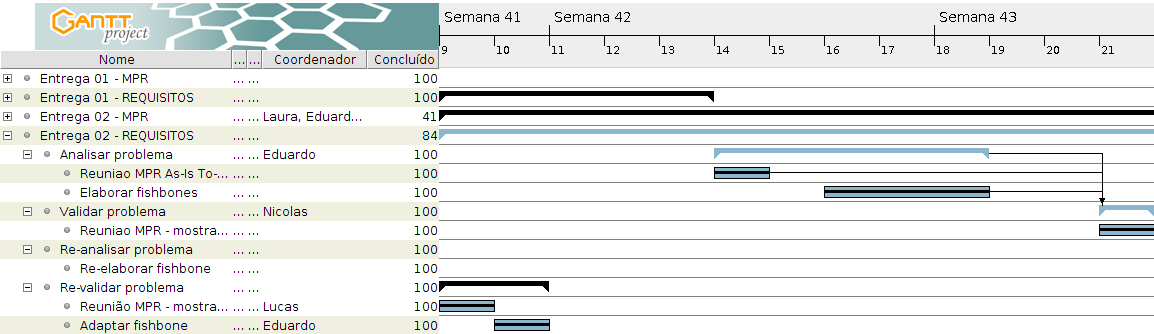
\includegraphics[width=\textwidth]{figuras/cronograma1}
    \caption{Cronograma das atividades: 09/10 - 29/10}
    \label{fig:cronograma1}
  \end{figure}

  \begin{figure}[H]
    \centering
    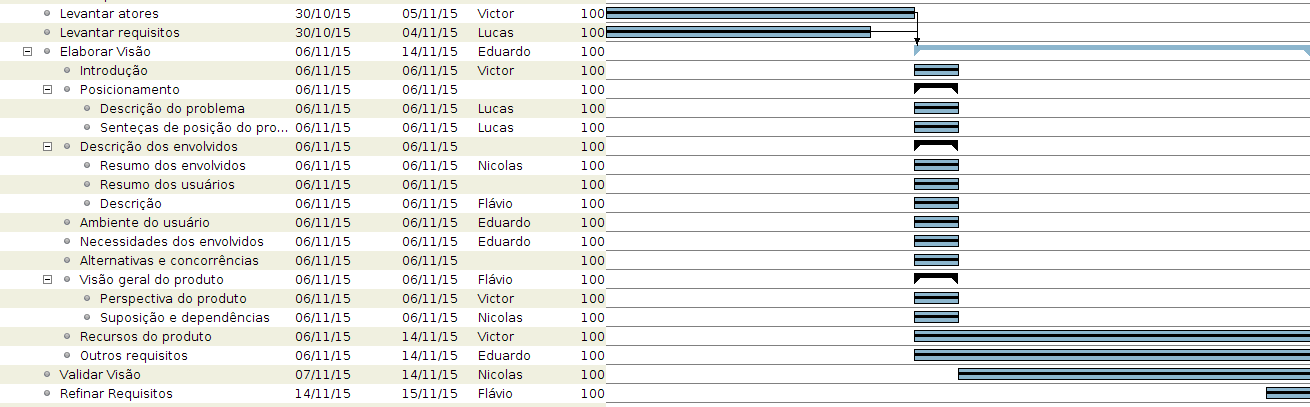
\includegraphics[width=\textwidth]{figuras/cronograma2}
    \caption{Cronograma das atividades: 30/10 - 15/11}
    \label{fig:cronograma2}
  \end{figure}

  \begin{figure}[H]
    \centering
    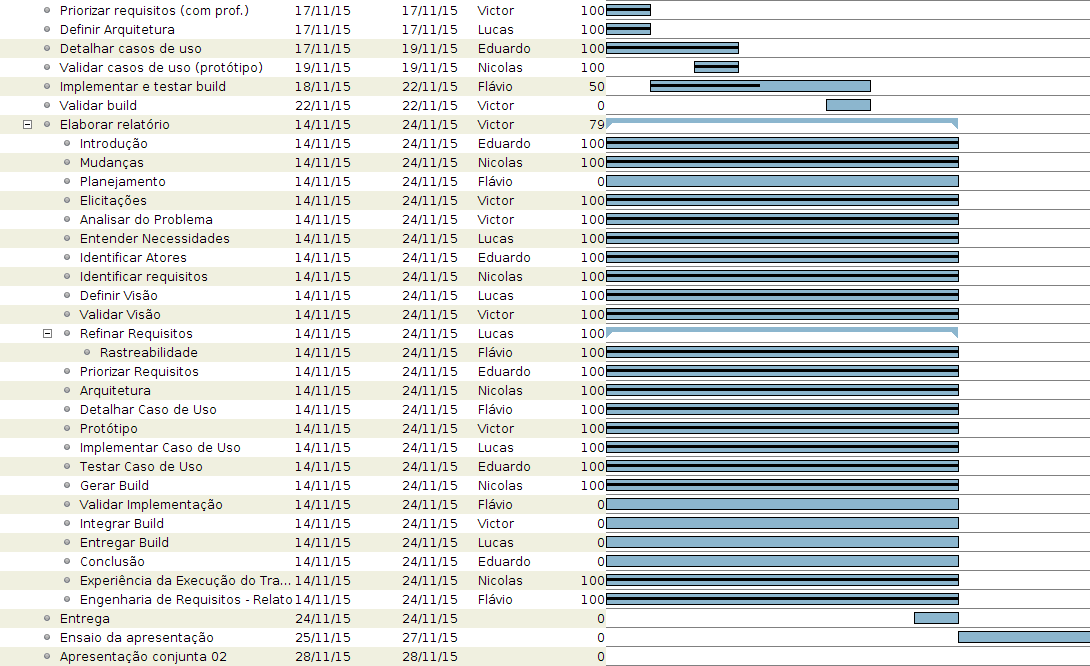
\includegraphics[width=\textwidth]{figuras/cronograma3}
    \caption{Cronograma das atividades: 16/11 - 28/11}
    \label{fig:cronograma3}
  \end{figure}
